\documentclass[hyperref=unicode,presentation,10pt]{beamer}

\usepackage[absolute,overlay]{textpos}
\usepackage{array}
\usepackage{graphicx}
\usepackage{adjustbox}
\usepackage[version=4]{mhchem}
\usepackage{chemfig}
\usepackage{caption}

%dělení slov
\usepackage{ragged2e}
\let\raggedright=\RaggedRight
%konec dělení slov

\addtobeamertemplate{frametitle}{
   \let\insertframetitle\insertsectionhead}{}
\addtobeamertemplate{frametitle}{
   \let\insertframesubtitle\insertsubsectionhead}{}

\makeatletter
  \CheckCommand*\beamer@checkframetitle{\@ifnextchar\bgroup\beamer@inlineframetitle{}}
  \renewcommand*\beamer@checkframetitle{\global\let\beamer@frametitle\relax\@ifnextchar\bgroup\beamer@inlineframetitle{}}
\makeatother
\setbeamercolor{section in toc}{fg=red}
\setbeamertemplate{section in toc shaded}[default][100]

\usepackage{fontspec}
\usepackage{unicode-math}

\usepackage{polyglossia}
\setdefaultlanguage{czech}

\def\uv#1{„#1“}

\mode<presentation>{\usetheme{default}}
 \usecolortheme{crane}

\setbeamertemplate{footline}[frame number]

\title[Crisis]
{C2062 -- Anorganická chemie II}

\subtitle{Vanad, niob, tantal a dubnium}
\author{Zdeněk Moravec, hugo@chemi.muni.cz \\ 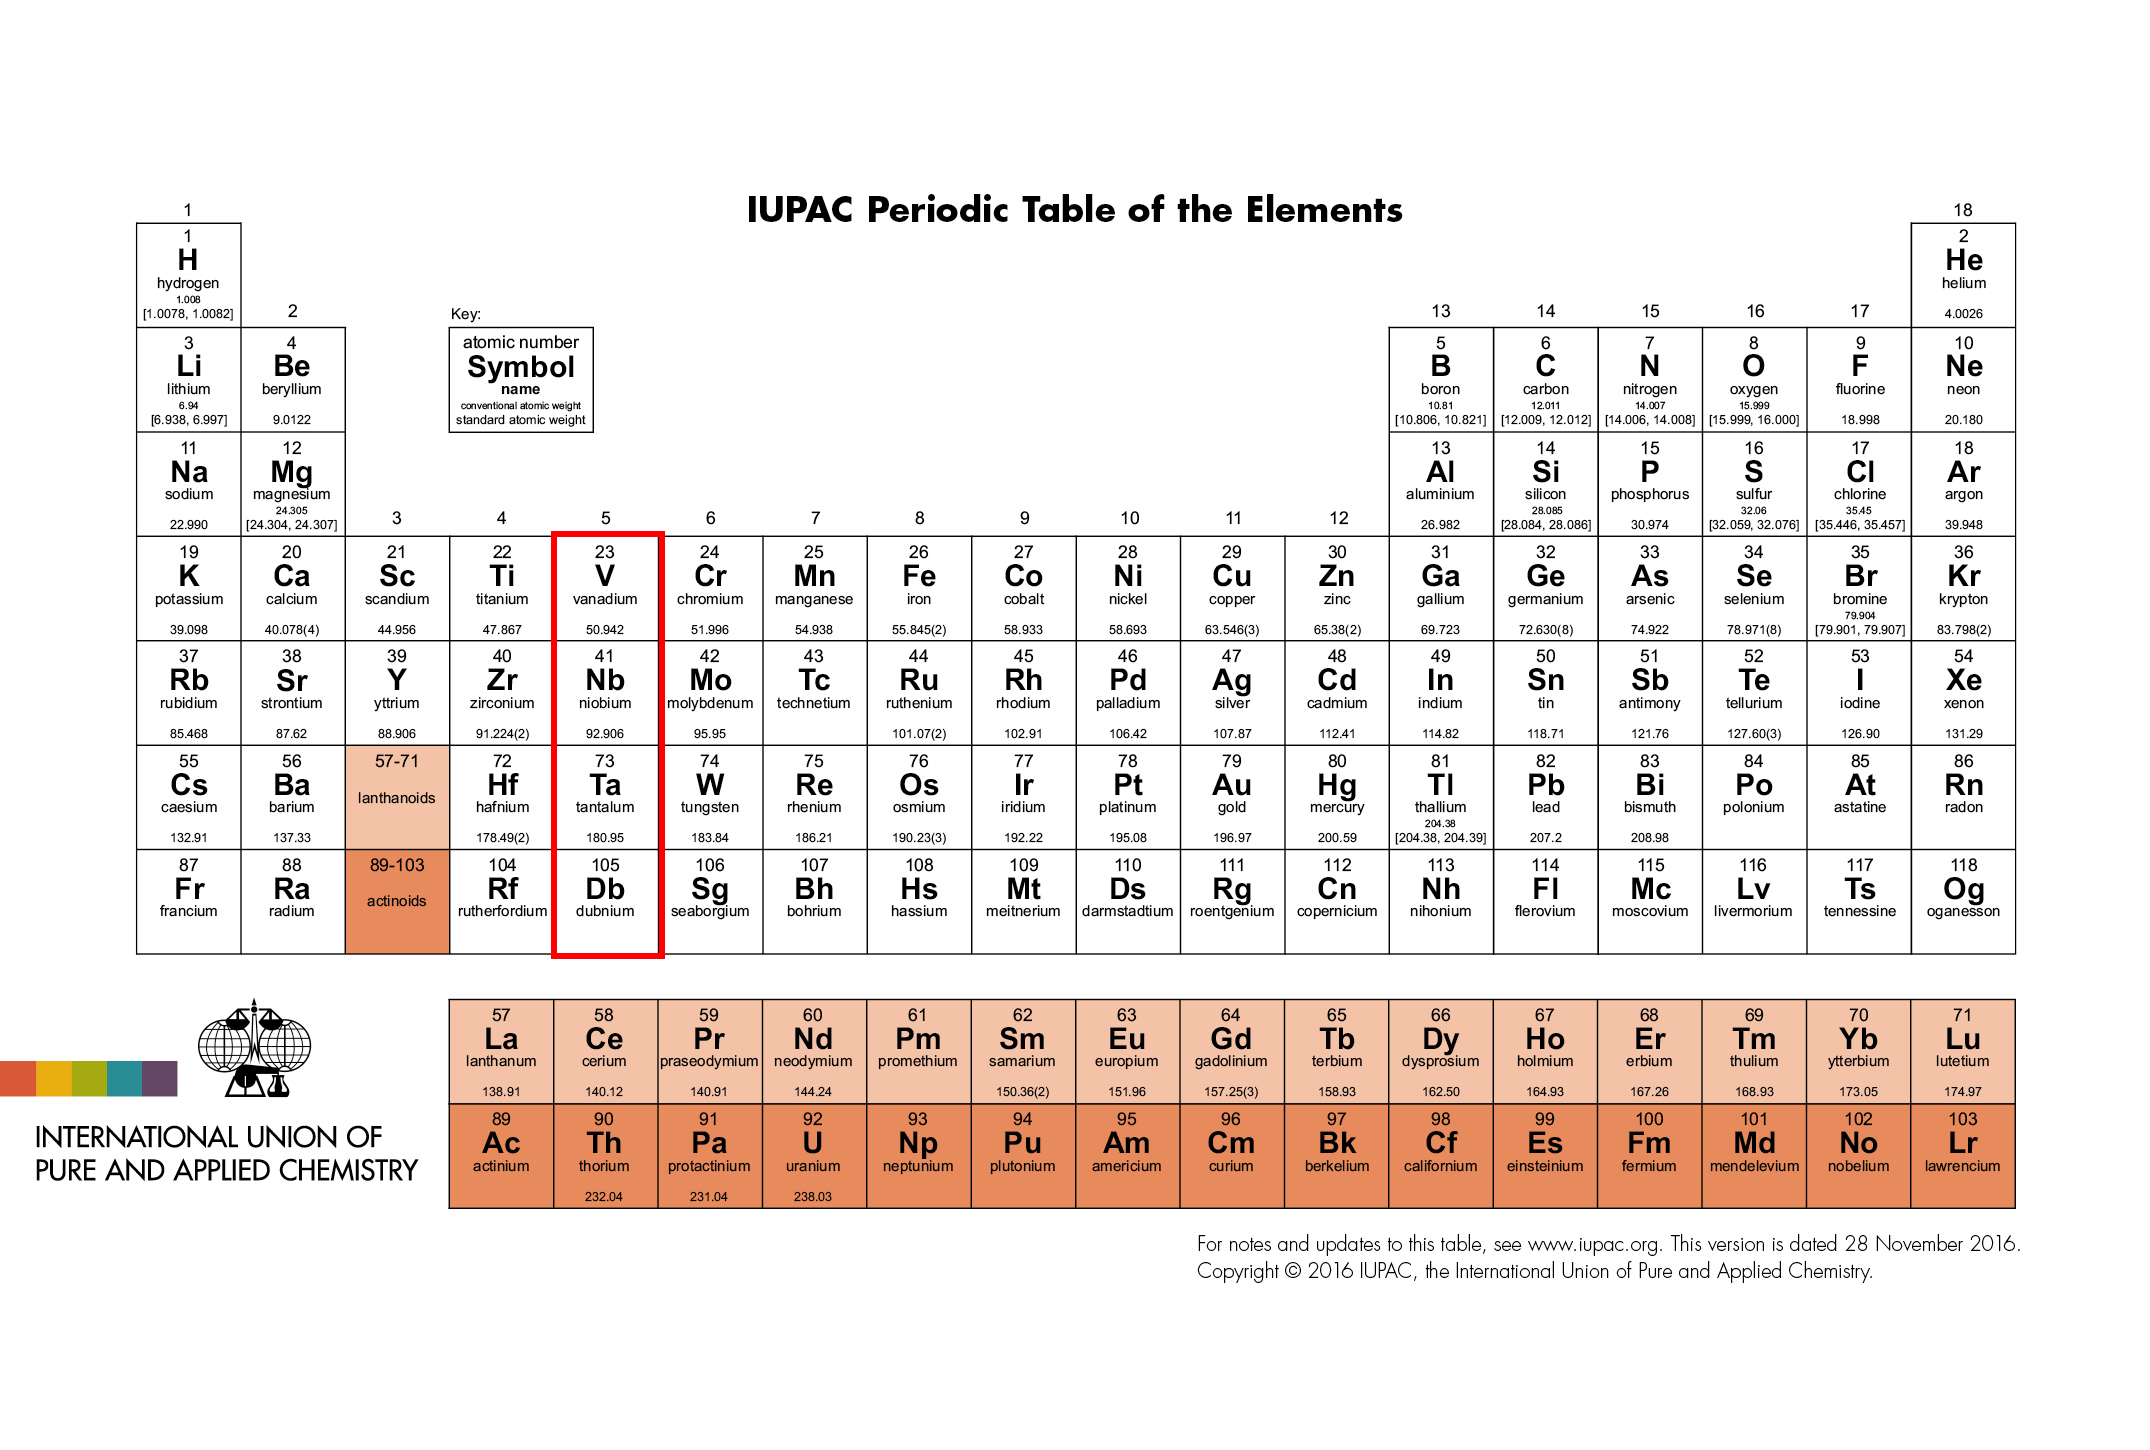
\includegraphics[height=60mm]{img/IUPAC_PSP.jpg}}
\date{}

\begin{document}
\begin{frame}
	\titlepage
\end{frame}

\section{Úvod}
\frame{
	\frametitle{}
	\vfill
	\begin{tabular}{|l|l|l|l|}
	\hline
	 & \textit{Vanad} & \textit{Niob} & \textit{Tantal} \\\hline
	 El. k. & 3d$^{3}$ 4s$^{2}$ & 4d$^{4}$ 5s$^{1}$ & 4f$^{14}$ 5d$^{3}$ 6s$^{2}$ \\\hline
	 T$_v$ [$^\circ$C] & 3407 & 4744 & 5458 \\\hline
	 T$_t$ [$^\circ$C] & 1910 & 2477 & 3017 \\\hline
	 Objev & 1831 & 1801 & 1802 \\\hline
	 & modrostříbrný\footnote[frame]{Zdroj: \href{https://commons.wikimedia.org/wiki/File:Vanadium-pieces.jpg}{Jurii/Commons}} & šedý\footnote[frame]{Zdroj: \href{https://commons.wikimedia.org/wiki/File:Niobium_rod.jpg}{W. Oelen/Commons}} & šedomodrý\footnote[frame]{Zdroj: \href{https://commons.wikimedia.org/wiki/File:73--tantalum,_foil.JPG}{Silverhill/Commons}} \\
	 & \begin{minipage}{.2\textwidth}
	 	\adjincludegraphics[width=\linewidth]{img/Vanadium.jpg}
	 \end{minipage}
	 	& \begin{minipage}{.2\textwidth}
	 		\adjincludegraphics[width=\linewidth]{img/Niobium_rod.jpg}
	 	\end{minipage} & \begin{minipage}{.2\textwidth}
	 	\adjincludegraphics[width=\linewidth]{img/tantalum_foil.jpg} \end{minipage} \\\hline
	\end{tabular}
	\vfill
}

\frame{
	\frametitle{}
	\vfill
	\begin{columns}
		\begin{column}{.7\textwidth}
		\textbf{Dubnium}
		\begin{itemize}
		\item Umělý prvek, transuran, protonové číslo 105, Db.
		\item Poprvé byl připraven v roce 1968 v~Dubně:
		\item \ce{^{243}_{95}Am + ^{22}_{10}Ne -> ^{261}_{105}Db + 4 n}
		\item \ce{^{243}_{95}Am + ^{22}_{10}Ne -> ^{260}_{105}Db + 5 n}
		\item Název prvku byl schválen roku 1997, odkazuje na ruské město Dubna.\footnote[frame]{\href{https://doi.org/10.1351/pac199769122471}{Names and symbols of transfermium elements (IUPAC Recommendations 1997)}}
		\item Nejstabilnějším izotopem je \ce{^{268}Db} s~poločasem rozpadu 16~hodin.\footnote[frame]{\href{https://doi.org/10.1103/PhysRevC.106.L031301}{First experiment at the Super Heavy Element Factory: High cross section of \ce{^{288}Mc} in the  \ce{^{243}Am + ^{48}Ca} reaction and identification of the new isotope \ce{^{264}Lr}}}
		\end{itemize}
		\begin{center}
		\begin{tabular}{|l|l|}
			\hline
			$^{266}$Db & 11 min \\\hline
			$^{267}$Db & 1,4 h \\\hline
			$^{268}$Db & 16 h \\\hline
		\end{tabular}
		\end{center}
		\end{column}
		\begin{column}{.3\textwidth}
			\begin{figure}
				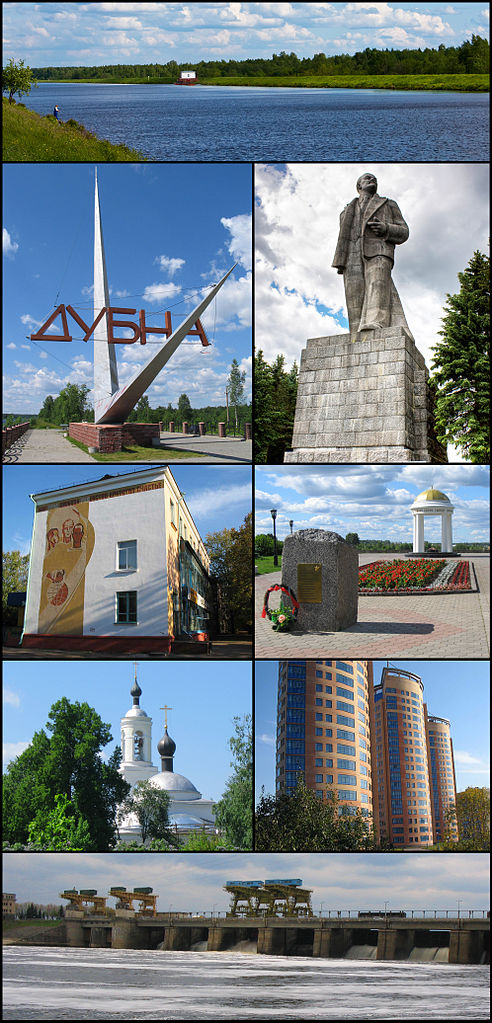
\includegraphics[height=.6\textheight]{img/Dubna_Collage.jpg}
				\caption*{Dubna.\footnote[frame]{\href{https://commons.wikimedia.org/wiki/File:Dubna\_Collage.jpg}{Zdroj: Pankratov-p/Commons}}}
			\end{figure}
		\end{column}
	\end{columns}
	\vfill
}

\section{Chemické a fyzikální vlastnosti}
\frame{
	\frametitle{}
	\vfill
	\begin{itemize}
		\item Elektronová konfigurace niobu je odlišná od vanadu a tantalu:
			\begin{itemize}
				\item 4d$^4$ 5s$^1$
			\end{itemize}
		\item Všechny tři kovy jsou stříbrolesklé a krystalují v kubické, plošně centrované mřížce (FCC).
		\item V čistém stavu jsou měkké a tažné, nečistoty způsobují tvrdost a~křehkost.
		\item Vlastnosti prvků jsou podobné prvkům 4. skupiny.
		\item Kovový vanad je silné redukční činidlo.
		\item Na vzduchu se pasivují tvorbou oxidické vrstvy.
		\item Rozpouštějí se v oleu, kyselině fluorovodíkové a ve směsi \ce{HF/HNO3}.
		\item Niob a tantal se rozpouštějí i v dalších minerálních kyselinách.
		\item Vytvářejí sloučeniny v rozmezí oxidačních čísel -III až V.
		\item Koordinační číslo může dosahovat až hodnoty 8.
	\end{itemize}
	\vfill
}

\section{Výskyt a získávání prvků}
\subsection{Vanad}
\frame{
	\frametitle{}
	\vfill
	\begin{itemize}
		\item Koncentrace vanadu v zemské kůře je přibližně 136 ppm, čímž se řadí mezi Zr a Cl.
		\item I přes relativně vysoké zastoupení se vanad vyskytuje v přírodě vzácně, jen v malých množstvích.
		\item Je známo téměř 200 minerálů obsahujících vanad, ale bohatší naleziště jsou vzácná.\footnote[frame]{\href{https://www.mindat.org/element/Vanadium}{The mineralogy of Vanadium}}
		\item Nejdůležitějšími minerály jsou \textit{patronit}, \textit{vanadinit} a \textit{karnotit}.
		\item Vanad se získává jako vedlejší produkt jiných procesů, např. zpracování bauxitu.
		\item Jedním z důležitých zdrojů jsou popílky vznikající destilací ropy.
		\item V roce 2017 bylo celosvětově vyrobeno více než 71 miliónů tun vanadu.\footnote[frame]{\href{https://www.usgs.gov/centers/nmic/vanadium-statistics-and-information}{Vanadium Statistics and Information}}
	\end{itemize}
	\vfill
}

\frame{
	\frametitle{}
	\vfill
	\textbf{Patronit}
	\begin{itemize}
		\item Jednoklonný minerál, \ce{VS4}. Chemicky se jedná o disulfid vanadičitý, \ce{V(S2)2}.\footnote[frame]{\href{https://rruff.info/doclib/hom/patronite.pdf}{Patrónite -- mineral data}}
		\item Je podobný grafitu, má černou až tmavě hnědou barvu. Na řezu je šedý.\footnote[frame]{\href{https://www.mindat.org/min-3131.html}{Patrónite}}
	\end{itemize}
	\begin{figure}
		\adjincludegraphics[height=.4\textheight]{img/Patronite.jpg}
		\caption*{Patronit.\footnote[frame]{Zdroj: \href{https://commons.wikimedia.org/wiki/File:Patrónite_-_Mineralogisches_Museum_Bonn.jpg}{Ra'ike/Commons}}}
	\end{figure}
	\vfill
}

\frame{
	\frametitle{}
	\vfill
	\textbf{Vanadinit}
	\begin{itemize}
		\item Hexagonální minerál, \ce{Pb5(VO4)3Cl}.\footnote[frame]{\href{https://mineraly.sci.muni.cz/fosfaty/vanadinit.html}{Vanadinit}}
		\item Slouží jako komerční zdroj pro přípravu vanadu a minoritně také olova.
		\item Poprvé byl objeven v roce 1801 v Mexiku.\footnote[frame]{\href{https://www.mindat.org/min-4139.html}{Vanadinite}}
	\end{itemize}
	\begin{columns}
		\begin{column}{.5\textwidth}
		\begin{figure}
			\adjincludegraphics[height=.32\textheight]{img/Vanadinite.jpg}
			\caption*{Vanadinit, Maroko.\footnote[frame]{Zdroj: \href{https://commons.wikimedia.org/wiki/File:Vanadinite_-_ACF_mine,_Mibladen,_Morocco.jpg}{Ivar Leidus/Commons}}}
		\end{figure}
		\end{column}

		\begin{column}{.5\textwidth}
			\begin{figure}
				\adjincludegraphics[height=.32\textheight]{img/Vanadinit2.jpg}
				\caption*{Vanadinit, muzeum Bonn.\footnote[frame]{Zdroj: \href{https://commons.wikimedia.org/wiki/File:Vanadinit_-_Mineralogisches_Museum_Bonn_(7275).jpg}{Raimond Spekking/Commons}}}
			\end{figure}
		\end{column}
	\end{columns}
	\vfill
}

\frame{
	\frametitle{}
	\vfill
	\textbf{Karnotit}
	\begin{itemize}
		\item Jednoklonný minerál, \ce{K2(UO2)2(VO4)2.3H2O}. Obsah vody bývá proměnlivý a často obsahuje malá množství dalších kovů: Ca, Ba, Fe, Mg nebo Na.\footnote[frame]{\href{https://rruff.info/doclib/hom/carnotite.pdf}{Carnotite -- mineral data}}
		\item Je zeleno-žlutý a využívá se jako ruda uranu a vanadu.\footnote[frame]{\href{https://www.mindat.org/min-907.html}{Carnotite}}
	\end{itemize}
	\begin{columns}
	\begin{column}{.5\textwidth}
		\begin{figure}
			\adjincludegraphics[width=.8\textwidth]{img/Carnotit.jpg}
			\caption*{Carnotit, Utah.\footnote[frame]{Zdroj: \href{https://commons.wikimedia.org/wiki/File:Carnotit_auf_fossilisiertem_Holz_-_St-George,_Utah.jpg}{Ra'ike/Commons}}}
		\end{figure}
	\end{column}

	\begin{column}{.5\textwidth}
		\begin{figure}
			\adjincludegraphics[width=.8\textwidth]{img/Carnotite-96138.jpg}
			\caption*{Carnotit, Kongo.\footnote[frame]{Zdroj: \href{https://commons.wikimedia.org/wiki/File:Carnotite-96138.jpg}{Leon Hupperichs/Commons}}}
		\end{figure}
	\end{column}
	\end{columns}
	\vfill
}

\frame{
	\frametitle{}
	\vfill
	\begin{itemize}
		\item Vanad se z rud získává pražením drtě s NaCl nebo \ce{Na2CO3} při teplotě 850~$^\circ$C.
		\item Získaný roztok obsahující metavadičnan sodný (\ce{NaVO3}) je okyselen, čímž se vysráží polyvanadičnany (červený koláč).
		\item Ten je následně redukován kovovým vápníkem nebo hořčíkem.
		\item Čistý vanad se získává van Arkel--de Boerovým procesem, tj. rozkladem těkavého jodidu:\footnote[frame]{\href{https://iopscience.iop.org/article/10.1149/1.2428019}{Preparation of High‐Purity Vanadium Metal by the Iodide Refining Process}}
		\item \ce{2 V + 3 I2 ->[850 $^\circ$C] 2 VI3}
		\item \ce{2 VI3 ->[1000 $^\circ$C] 2 V + 3 I2}
	\end{itemize}
	\vfill
}

\frame{
	\frametitle{}
	\vfill
	\begin{figure}
		\adjincludegraphics[height=.65\textheight]{img/Van-Arkel-de-Boer-Apparat.png}
		\caption*{1 - přívod vakua; 2 - molybdenová elektroda; 3 - molybdenová síť; 4 - zásobník surového materiálu; 5 - wolframové vlákno\footnote[frame]{Zdroj: \href{https://commons.wikimedia.org/wiki/File:Van-Arkel-de-Boer-Apparat.png}{	Roland Mattern/Commons}}}
	\end{figure}
	\vfill
}

\subsection{Niob, tantal}
\frame{
	\frametitle{}
	\vfill
	\begin{itemize}
		\item Koncentrace niobu v zemské kůře je přibližně 20 ppm, je 34. nejrozšířenější prvek.
		\item Koncentrace tantalu v zemské kůře je přibližně 1,7 ppm.
		\item Čistý niob se v přírodě nevyskytuje, minerály obsahující niob obsahují zpravidla i tantal.
		\item Nejdůležitějším minerálem je \ce{(Fe,Mn)(Nb,Ta)2O6}, pokud obsahuje více niobu označuje se jako \textit{kolumbit}, v případě nadbytku tantalu jde o \textit{tantalit}.\footnote[frame]{\href{http://geologie.vsb.cz/loziska/suroviny/rudy/columbit.html}{COLUMBIT - skupinové jméno pro minerály se vzorcem \ce{(Fe,Mn)(Nb,Ta)2O6}}}
		\item Stejně jako u vanadu, nenacházíme bohatší naleziště ani u těchto prvků.
	\end{itemize}
	\vfill
}

\frame{
	\frametitle{}
	\vfill
	\textbf{Kolumbit}
	\begin{itemize}
		\item Orthorombický minerál, \ce{Fe^{2+}Nb2O6}.
		\item Má černou až hnědočernou barvu.\footnote[frame]{\href{https://www.mindat.org/min-1514.html}{Columbite-(Fe)}}
	\end{itemize}
	\begin{columns}
		\begin{column}{.5\textwidth}
			\begin{figure}
				\adjincludegraphics[width=.6\textwidth]{img/Columbite-162793.jpg}
				\caption*{Columbit, USA.\footnote[frame]{Zdroj: \href{https://commons.wikimedia.org/wiki/File:Carnotite-96138.jpg}{Robert M. Lavinsky/Commons}}}
			\end{figure}
		\end{column}

		\begin{column}{.5\textwidth}
			\begin{figure}
				\adjincludegraphics[width=.6\textwidth]{img/Columbite-75444.jpg}
				\caption*{Columbit, USA.\footnote[frame]{Zdroj: \href{https://commons.wikimedia.org/wiki/File:Columbite-75444.jpg}{Robert M. Lavinsky/Commons}}}
			\end{figure}
		\end{column}
	\end{columns}
	\vfill
}

\frame{
	\frametitle{}
	\vfill
	\textbf{Tantalit}
	\begin{itemize}
		\item Orthorombický minerál, \ce{(Fe,Mn)Ta2O6}.\footnote[frame]{\href{https://mineraly.sci.muni.cz/oxidy/tantalit.html}{Tantalit}}
		\item Má černou až načervenalou barvu.\footnote[frame]{\href{https://www.mindat.org/min-3882.html}{Tantalite}}
	\end{itemize}
	\begin{columns}
		\begin{column}{.5\textwidth}
			\begin{figure}
				\adjincludegraphics[width=.8\textwidth]{img/Tantalite.jpg}
				\caption*{Tantalit, USA.\footnote[frame]{Zdroj: \href{https://commons.wikimedia.org/wiki/File:Tantalite.jpg}{Andrew Silver/Commons}}}
			\end{figure}
		\end{column}

		\begin{column}{.5\textwidth}
			\begin{figure}
				\adjincludegraphics[width=.8\textwidth]{img/Tantalite-272645.jpg}
				\caption*{Tantalit, Brazílie.\footnote[frame]{Zdroj: \href{https://commons.wikimedia.org/wiki/File:Tantalite-272645.jpg}{Robert M. Lavinsky/Commons}}}
			\end{figure}
		\end{column}
	\end{columns}
	\vfill
}

\frame{
	\frametitle{}
	\vfill
	\textbf{Samarskit-(Y)}
	\begin{itemize}
		\item Orthorombický minerál, \ce{(YFe^{3+}Fe^{2+}U,Th,Ca)2(Nb,Ta)2O8}.\footnote[frame]{\href{https://www.mindat.org/min-3512.html}{Samarskite-(Y)}}
		\item Má černou až hnědou barvu.
	\end{itemize}
	\begin{columns}
		\begin{column}{.5\textwidth}
			\begin{figure}
				\adjincludegraphics[width=.8\textwidth]{img/Samarskite.jpg}
				\caption*{Samarskit, USA.\footnote[frame]{Zdroj: \href{https://commons.wikimedia.org/wiki/File:Samarskite.jpg}{Andrew Silver/Commons}}}
			\end{figure}
		\end{column}

		\begin{column}{.5\textwidth}
			\begin{figure}
				\adjincludegraphics[width=.5\textwidth]{img/Samarskite-75446.jpg}
				\caption*{Samarskit, USA.\footnote[frame]{Zdroj: \href{https://commons.wikimedia.org/wiki/File:Samarskite-(Y)-75446.jpg}{Robert M. Lavinsky/Commons}}}
			\end{figure}
		\end{column}
	\end{columns}
	\vfill
}

\frame{
	\frametitle{}
	\vfill
	\textbf{Fergusonit}
	\begin{itemize}
		\item Orthorombický minerál, \ce{(Y,REE)NbO4} (REE - Rare-Earth Elements).\footnote[frame]{\href{http://webmineral.com/data/Fergusonite-(Y).shtml}{Fergusonite-(Y) Mineral Data}}
		\item Má černou až šedou barvu, může být i žlutý.
	\end{itemize}
	\begin{columns}
		\begin{column}{.5\textwidth}
			\begin{figure}
				\adjincludegraphics[width=.8\textwidth]{img/Fergusonit.jpg}
				\caption*{Fergusonit, Švédsko.\footnote[frame]{Zdroj: \href{https://commons.wikimedia.org/wiki/File:Fergusonit.jpg}{Alchemist-hp/Commons}}}
			\end{figure}
		\end{column}

		\begin{column}{.5\textwidth}
			\begin{figure}
				\adjincludegraphics[width=.8\textwidth]{img/Fergusonite-135271.jpg}
				\caption*{Fergusonit, Madagaskar.\footnote[frame]{Zdroj: \href{https://commons.wikimedia.org/wiki/File:Fergusonite-(Y)-135271.jpg}{Robert M. Lavinsky/Commons}}}
			\end{figure}
		\end{column}
	\end{columns}
	\vfill
}

\frame{
	\frametitle{}
	\vfill
	\begin{itemize}
		\item Niob i tantal se vyrábějí v menším množství než vanad.
		\item Z minerálů se izoluje směs oxidů \ce{Nb2O5} a \ce{Ta2O5}.
		\item Tato směs pak reaguje s kyselinou fluorovodíkovou.
		\item \ce{Ta2O5 + 14 HF -> 2 H2[TaF7] + 5 H2O}
		\item \ce{Nb2O5 + 10 HF -> 2 H2[NbOF5] + 3 H2O}
		\item Kovy jsou pak separovány extrakcí pomocí ketonů, např. cyklohexanonu.\footnote[frame]{\href{https://doi.org/10.1021/ie50623a016}{STAFF-INDUSTRY COLLABORATIVE REPORT Tantalum and Niobium}}
		\item Redukci oxidů lze provést několika metodami:
		\begin{itemize}
			\item Redukce vodíkem nebo uhlíkem.
			\item Elektrolýzou taveniny \ce{K2[NbOF5]} a chloridu sodného.
			\item Aluminotermickou reakcí oxidu niobičného nebo směsi oxidů:
			\item \ce{3 Nb2O5 + Fe2O3 + 12 Al -> 6 Nb + 2 Fe + 6 Al2O3}
			\item Tímto procesem získáme slitinu ferroniob nebo ferrotantal.\footnote[frame]{\href{https://www.usgs.gov/centers/nmic/ferroalloys-statistics-and-information}{Ferroalloys Statistics and Information}}
		\end{itemize}
	\end{itemize}
	\vfill
}

\section{Využití prvků}
\subsection{Vanad}
\frame{
	\frametitle{}
	\vfill
	\begin{itemize}
		\item Hlavní využití nachází vanad jako příměs do ocelí (\textit{ferrovanad}).
		\item S uhlíkem v oceli vytváří jemná zrna \ce{V4C3}, ta jsou rozptýlena v~objemu a dávají oceli vyšší odolnost vůči opotřebení, a to i za vysokých teplot.
		\item Tyto oceli se využívají při konstrukci pružin a rychlořezných ocelí.
		\item Obsah vanadu se pohybuje mezi 35 a 80~\%.
		\item Nejběžnějším typem ferrovanadu je FeV80, který obsahuje 80~\% vanadu.
		\item Vyrábí se z oxidu vanadičného redukcí ferrosiliciem nebo hliníkem.
		\item Jako struskotvorná látka se využívá pálené vápno.
	\end{itemize}
	\begin{align*}
		\ce{3 V2O5 + 10 Al &-> 6 V + 5 Al2O3} \\
		\ce{2 V2O5 + 5 Si + 10 CaO &-> 4 V + 5 Ca2SiO4} \\
		\ce{V_x + Fe_{1-x} &-> (Fe_{1-x}V_x)}
	\end{align*}
	\vfill
}

\frame{
	\frametitle{}
	\vfill
	\begin{itemize}
		\item Další významné využití vanadu je v katalýze.\footnote[frame]{\href{https://doi.org/10.1021/acs.chemrev.8b00245}{Catalytic Applications of Vanadium: A Mechanistic Perspective}}
		\item Oxid vanadičný, \ce{V2O5}, katalyzuje oxidaci oxidu siřičitého na sírový při kontaktní výrobě kyseliny sírové za teploty 430~$^\circ$C.\footnote[frame]{\href{https://doi.org/10.1006/jcat.1995.1185}{Deactivation and Compound Formation in Sulfuric-Acid Catalysts and Model Systems}}
		\item \ce{V2O5 + SO2 -> 2 VO2 + SO3}
		\item \ce{4 VO2 + O2 -> 2 V2O5}
		\item K oxidaci \textit{n}-butanu na maleinanhydrid se používá tzv. \textit{VPO katalyzátor}.\footnote[frame]{\href{https://doi.org/10.1006/jcat.1995.1228}{Evolution of a VPO Catalyst in n-Butane Oxidation Reaction During the Activation Time}} Ten se připravuje reakcí \ce{V2O5} s \ce{H3PO4}.
	\end{itemize}
	\begin{figure}
		\adjincludegraphics[width=\textwidth]{img/VPO.png}
	\end{figure}
	\vfill
}

\frame{
	\frametitle{}
	\vfill
	\begin{itemize}
		\item Vanadové redoxní baterie jsou typem průtočných baterií, mohou být velmi významnou technologií pro zálohování obnovitelných zdrojů elektrické energie.\footnote[frame]{\href{https://www.vscht.cz/popularizace/doktorandi-pisou/kam-s-elektrinou}{Kam s elektřinou? Řešením mohou být vanadové průtočné baterie}}
		\item Výhodou těchto baterií je snadná škálovatelnost, ve srovnání se statickými články. Kapacita baterie je dána objemem elektrolytu a její výkon je dán povrchem elektrod a počtem článků.
		\item Elektrolyt v kladném poločlánku je tvořen ionty \ce{VO$_2^+$} a \ce{VO^{2+}} a v záporné pak \ce{V^{2+}} a \ce{V^{3+}}. Lze jej připravit elektrolytickým rozpouštěním \ce{V2O5} v kyselině sírové.
	\end{itemize}
	\begin{figure}
		\adjincludegraphics[height=.35\textheight]{img/Vanadium_Redox_flow_battery.jpg}
	\end{figure}
	\vfill
}

\frame{
	\frametitle{}
	\vfill
	\begin{figure}
		\adjincludegraphics[height=.7\textheight]{img/Redox_Flow_Battery.jpg}
		\caption*{Schéma redoxní průtokové baterie.\footnote[frame]{\href{https://commons.wikimedia.org/wiki/File:Redox_Flow_Battery.jpg}{Zdroj: Colintheone/Commons}}}
	\end{figure}
	\vfill
}

\frame{
	\frametitle{}
	\vfill
	\begin{itemize}
		\item V roce 2022 Čína zprovoznila v Ta-lienu největší baterii tohoto typu, jako úložiště pro elektřinu získávanou z obnovitelných zdrojů (slunce a větru).\footnote[frame]{\href{https://www.svethardware.cz/cina-spustila-nejvetsi-redox-flow-baterii-na-svete-se-100mw-400mwh/58424}{Čína spustila největší redox flow baterii na světě se 100MW/400MWh}}
		\item Baterie dokáže uložit 400 MWh energie a do sítě zvládne dodávat 100 MW.\footnote[frame]{\href{https://www.pv-magazine.com/2022/09/29/china-connects-worlds-largest-redox-flow-battery-system-to-grid/}{China connects world’s largest redox flow battery system to grid
		}}
		\item Je plánováno v budoucnu zvýšit tyto parametry na dvojnásobek.
	\end{itemize}
	\begin{figure}
		\adjincludegraphics[width=\textwidth]{img/Dalian_pan.jpg}
		\caption*{Ta-lien.\footnote[frame]{\href{https://commons.wikimedia.org/wiki/File:Dalian_pan.jpg}{Zdroj: Michael Saechang/Commons}}}
	\end{figure}
	\vfill
}

\frame{
	\frametitle{}
	\vfill
	\begin{itemize}
		\item Slitina \ce{V3Ga} je supravodivá, její kritická teplota je 14,2~K a kritické magnetické pole 19~T.\footnote[frame]{\href{https://doi.org/10.1109/TMAG.1977.1059431}{A 17.5 Tesla superconducting concentric Nb3Sn and V3Ga magnet system}}
		\item Díky těmto parametrů se využívá pro konstrukci supravodivých magnetů pro vysoká pole.
	\end{itemize}

	\begin{figure}
		\adjincludegraphics[height=.4\textheight]{img/V3GaWire.jpg}
		\caption*{Supravodivý drát z \ce{V3Ga}.\footnote[frame]{\href{https://commons.wikimedia.org/wiki/File:V3GaWire.jpg}{Zdroj: Materialscientist/Commons}}}
	\end{figure}
	\vfill
}

\subsection{Niob}
\frame{
	\frametitle{}
	\vfill
	\begin{columns}
		\begin{column}{.6\textwidth}
		\begin{itemize}
		\item Supravodivé dráty NbTi se využívají v MRI (Magnet Resonance Imaging) magnetech a také v magnetech u LHC. Kritická teplota je okolo 10~K a hodnota kritického pole dosahuje 15~T.\footnote[frame]{\href{https://doi.org/10.1016/0011-2275(87)90057-9}{Emergence of Nb-Ti as supermagnet material}}
		\item Další důležité slitiny jsou \ce{Nb3Ge}\footnote[frame]{\href{https://www.osti.gov/biblio/928774-D1NAve/}{Limits of NbTi and \ce{Nb3Sn}, and Development of W\&R Bi-2212 HighField Accelerator Magnets}} a \ce{Nb3Sn},\footnote[frame]{\href{https://doi.org/10.1007/BF00114941}{Preparation of \ce{Nb3Ge} films by chemical transport reaction and their critical properties}} které se využívají ke konstrukci supravodivých magnetů např. pro NMR a MRI.
		\item V reaktoru ITER bude využito zhruba 600 tun \ce{Nb3Sn} a 250 tun \ce{Nb3Ti}.
		\end{itemize}
	\end{column}
	\begin{column}{.4\textwidth}
		\begin{figure}
			\adjincludegraphics[width=\textwidth]{img/nmr300.jpg}
		\end{figure}
	\end{column}
	\end{columns}
	\vfill
}

\frame{
	\frametitle{}
	\vfill
	\begin{itemize}
		\item Slitiny niobu s dalšími kovy (Ti, Fe, Hf, Ta) se využívají v kosmických technologiích pro konstrukci trysek motorů na kapalné paliva.\footnote[frame]{\href{https://samario01.cbmm.com.br/cgs/publico/VisualizaArquivoBVPublica.ashx?DOC_Codigo=747}{Niobium Alloys and High Temperature Applications}}
		\item Např. slitina C103 byla využita v roce 1965 v programu Apollo.\footnote[frame]{\href{https://www.bayvillechemical.net/niobium-c-103-alloy}{Niobium C-103 Alloy}}
	\end{itemize}
	\begin{center}
		\begin{tabular}{|l|l|}
			\hline
			\textbf{Slitina} & \textbf{Složení} \\\hline
			C103 & 89 \% Nb, 10 \% Hf a 1 \% Ti \\\hline
			FS85 & 61 \% Nb, 10 \% W, 28 \% Ta a 1 \% Zr \\\hline
			Cb129Y & 79.8 \% Nb, 10 \% W, 10 \% Hf a 0.2 \% Y \\\hline
			Cb752 & 87.5 \% Nb, 10 \% W a 2.5 \% Zr \\\hline
			Nb1Zr & 99 \% Nb a 1 \% Zr \\\hline
		\end{tabular}
	\end{center}
	\vfill
}

\frame{
	\frametitle{}
	\vfill
	\begin{figure}
		\adjincludegraphics[height=.7\textheight]{img/Apollo_CSM_lunar_orbit.jpg}
		\caption*{Apollo 15 CSM.\footnote[frame]{Zdroj: \href{https://commons.wikimedia.org/wiki/File:Apollo_CSM_lunar_orbit.jpg}{NASA/Commons}}}
	\end{figure}
	\vfill
}

\frame{
	\frametitle{}
	\vfill
	\begin{columns}
		\begin{column}{.6\textwidth}
		\begin{itemize}
			\item Niobičnan lithný, \ce{LiNbO3}, je bezbarvý krystalický materiál.\footnote[frame]{\href{https://doi.org/10.1007/BF00614817}{Lithium niobate: Summary of physical properties and crystal structure}}
			\item Využívá se pro konstrukci piezoelektrických senzorů, optických modulátorů, optických vlnovodů, a dalších optických zařízení.
			\item Monokrystaly se připravují Czochralskiho metodou.
			\item Nanovlákna lze připravit hydrotermální reakcí oxidu niobičného s hydroxidem lithným v autoklávu při teplotě 150~$^\circ$C.\footnote[frame]{\href{https://doi.org/10.1063/1.3236777}{Lithium niobate nanowires synthesis, optical properties, and manipulation}}
			\item \ce{Nb2O5 + 2 LiOH -> 2 LiNbO3 + H2O}
		\end{itemize}
		\end{column}
		\begin{column}{.4\textwidth}
			\begin{figure}
				\adjincludegraphics[width=\textwidth]{img/Linbo3_Unit_Cell.png}
				\caption*{Krystalová struktura \ce{LiNbO3}.\footnote[frame]{Zdroj: \href{https://commons.wikimedia.org/wiki/File:Linbo3_Unit_Cell.png}{Ahellwig/Commons}}}
			\end{figure}
		\end{column}
	\end{columns}
	\vfill
}

\frame{
	\frametitle{}
	\vfill
	\begin{itemize}
		\item Jaderný izomer \ce{$^{93m}$Nb} se využívá jako zdroj RTG záření pro rentgenovou fluorescenci (XRF).\footnote[frame]{\href{https://doi.org/10.1016/0883-2889(90)90184-I}{The possibility of \ce{$^{93m}$Nb} radionuclide production in the nuclear reactor BR-10 ...}}
		\item Připravuje se ozařováním stabilního izotopu \ce{$^{93}$Nb} rychlými neutrony v jaderném reaktoru:
		\item \ce{$^{93}$Nb + n -> $^{93m}$Nb + n}
		\item Ozářený niob se nechá dostatečně dlouho stát, aby došlo k rozpadu izotopu \ce{$^{95}$Nb} (T$_\frac{1}{2}$ = 35 dnů) a pak se rozpustí ve směsi kyseliny fluorovodíkové a dusičné.
		\item \ce{$^{93}$Nb + n ->[][-$\gamma$] $^{94}$Nb + n ->[][-$\gamma$] $^{95}$Nb}
		\item Roztok se pak separuje na anexu.
		\item Deexcitace probíhá uvolněním fotonu o energii 30,8~keV, poločas přeměny 16,1 roku.
		\item Analogicky lze provést excitaci ozařováním niobu brzdným zářením o energii 5--30~MeV:
		\item \ce{$^{93}$Nb + $\gamma$ -> $^{93m}$Nb + $\gamma^\prime$}
	\end{itemize}
	\vfill
}

\subsection{Tantal}
\frame{
	\frametitle{}
	\vfill
	\begin{itemize}
		\item Tantal má hlavní využití v elektronice, využívá se při výrobě tantalových kondenzátorů.
		\item Oproti klasickým elektrolytickým kondenzátorům mají velmi výhodný poměr kapacity a objemu.
	\end{itemize}
	\begin{figure}
		\adjincludegraphics[height=.5\textheight]{img/Tantal-P1100196c.jpg}
		\caption*{Tantalové kondenzátory.\footnote[frame]{Zdroj: \href{https://commons.wikimedia.org/wiki/File:Tantal-P1100196c.jpg}{Jens Both/Commons}}}
	\end{figure}
	\vfill
}

\frame{
	\frametitle{}
	\vfill
	\begin{columns}
		\begin{column}{.75\textwidth}
			\begin{itemize}
				\item Anoda kondenzátoru je tvořena kovovým tantalem, vyrábí se lisováním práškového tantalu na tantalový drát ve vakuu při teplotě 1500--2000~$^\circ$C.\footnote[frame]{\href{https://www.avx.com/docs/techinfo/Tantalum-NiobiumCapacitors/bsctant.pdf}{Basic tantalum capacitor technology}}
				\item Kapacitance materiálu je závislá na měrném povrchu anody.
				\item Dielektrická vrstva se vyrábí elektrochemickou oxidací anody:
				\item \ce{2 Ta + 5 H2O -> Ta2O5 + 5 H2}
				\item Tloušťka dielektrické vrstvy určuje maximální napětí, které kondenzátor snese.
				\item Katoda je tvořena vrstvou \ce{MnO2} vytvořenou tepelným rozkladem dusičnanu manganatého.
				\item \ce{Mn(NO3)2 -> MnO2 + 2 NO2}
			\end{itemize}
		\end{column}
		\begin{column}{.25\textwidth}
			\begin{figure}
				\adjincludegraphics[width=\textwidth]{img/Parallel_plate_capacitor.png}
				\caption*{Schéma kondenzátoru.\footnote[frame]{Zdroj: \href{https://commons.wikimedia.org/wiki/File:Parallel_plate_capacitor.svg}{inductiveload/Commons}}}
			\end{figure}
		\end{column}
	\end{columns}
	\vfill
}

\frame{
	\frametitle{}
	\vfill
	\begin{figure}
		\adjincludegraphics[height=.7\textheight]{img/Tantalum_Capacitor_Production_Flow.png}
		\caption*{Výroba tantalových kondenzátorů.\footnote[frame]{Zdroj: \href{https://commons.wikimedia.org/wiki/File:Tantalum_Capacitor_Production_Flow.png}{Elcap/Commons}}}
	\end{figure}
	\vfill
}

\frame{
	\frametitle{}
	\vfill
	\begin{itemize}
		\item Tantal je také součástí mnoha slitin s vysokou teplotou tání, pevností a tažností.
		\item Využívají se pro speciální aplikace jako jsou tepelné výměníky, proudové motory, chemické a jaderné reaktory, atd.
		\item Tantal je odolný vůči působení kyselin, kromě HF a horké kyseliny sírové.
		\item Dokáže vázat kyslík a dusík (za tvorby oxidů a nitridů). Toho se využívá, při konstrukci vakuových elektronek, k udržování vysokého vakua.
		\item Vysoké teplotní stability se využívá i při konstrukci topných těles do vysokoteplotních pecí.
	\end{itemize}
	\vfill
}

\frame{
	\frametitle{}
	\vfill
	\begin{itemize}
		\item Izotop \textbf{\ce{$^{182}$Ta}} se připravuje ozařováním tantalu nebo oxidu tantaličného neutrony v jaderném reaktoru:
		\item \ce{$^{181}$Ta + n -> $^{182}$Ta + $\gamma$}
		\item Rozpadá se přeměnou $\beta^-$ s poločasem rozpadu 114,7 dní.
		\item \ce{$^{182}$Ta -> $^{182}$W + $\beta^-$}
		\item Tento izotop se ve formě \ce{^{182}Ta2O5} využívá pro monitorování výroby oceli a zjišťování původu oxidických vměstků.
		\item Využití nachází i v biologii, kde se využívají pouzdra s ozářeným tantalovým drátem pro monitorování pohybu malých živočichů (myší, mloků). Pouzdro je jim voperováno pod kůži.
	\end{itemize}
	\begin{figure}
		\adjincludegraphics[height=.3\textheight]{img/mlok.jpg}
		\caption*{Mlok skvrnitý.\footnote[frame]{Zdroj: \href{https://commons.wikimedia.org/wiki/File:Mlok.JPG}{Martin Filip + Tereza Procházková/Commons}}}
	\end{figure}
	\vfill
}

\section{Sloučeniny}
\frame{
	\frametitle{}
	\vfill
	\begin{itemize}
		\item Vanad a tantal mají elektronovou konfiguraci (n-1)d$^3$ ns$^2$. U niobu je konfigurace 4d$^4$ 5s$^1$.
		\item Vlastnosti prvků jsou podobné prvkům 4. skupiny.
		\item Na vzduchu se pasivují tvorbou oxidické vrstvy.
		\item Rozpouštějí se v oleu,\footnote[frame]{Dýmavá kyselina sírová, roztok oxidu sírového v kyselině sírové} kyselině fluorovodíkové a ve směsi \ce{HF/HNO3}.
		\item Niob a tantal se dále rozpouštějí i v dalších minerálních kyselinách.
		\item Vytvářejí sloučeniny v rozmezí oxidačních čísel -III až V.
		\item Koordinační číslo může dosahovat až hodnoty 8.
		\item Nejstabilnější oxidační číslo u vanadu je IV.
		\item Velmi stabilní je vanadylový kation \ce{VO^{2+}}, který obsahuje trojnou vazbu \ce{V\bond{3}O}.
		\item Známe také trihalogenidy vanadylu \ce{VOX3}.
		\item Niob a tantal mají velmi podobné chemické vlastnosti, preferují oxidační číslo V.
	\end{itemize}
	\vfill
}

\frame{
	\frametitle{}
	\vfill
	\begin{tabular}{|c|c|c|c|}
		\hline
		Ox. č. & K. č. & V & Nb/Ta \\\hline
		$-$III & 5 & \ce{[V(CO)5]^{3-}} & - \\\hline
		\hline
		$-$I & 6 & \ce{[V(CO)6]^{-}} & \ce{[M(CO)6]^{-}} \\\hline
		\hline
		0 & 6 & \ce{[V(CO)6]} & - \\\hline
		\hline
		I & 6 & \ce{[V(bipy)3]^+} & - \\\hline
		\hline
		II & 4 & - & NbO \\\hline
		& 6 & \ce{[V(CN)6]^{4-}} & \\\hline
		\hline
		III & 4 & \ce{[VCl4]^-} & - \\\hline
		& 8 & - & \ce{[Nb(CN)8]^{5-}} \\\hline
		\hline
		IV & 4 & \ce{VCl4} & \ce{[Nb(NEt2)4]} \\\hline
		& 5 & \ce{VO(acac)2} & - \\\hline
		& 6 & \ce{VCl4} & \ce{[Nb(NEt2)4]} \\\hline
		\hline
		V & 4 & \ce{VOCl3} & \ce{ScNbO4]} \\\hline
		& 5 & \ce{VCl5} & \ce{MF5} \\\hline
		& 6 & \ce{[VF6]^-} & \ce{[MF6]^-} \\\hline
		& 8 & \ce{[V(O2)4]^{3-}} & \ce{[M(O2)4]^{3-}} \\\hline
		&  &  & \ce{[MF8]^{-}} \\\hline
	\end{tabular}
	\vfill
}

\frame{
	\frametitle{}
	\vfill
	\begin{itemize}
		\item S $\pi$-akceptorními ligandy vytváří komplexní sloučeniny, kde vystupují v oxidačním čísle 0.
		\item Příkladem může být hexakarbonyl vanadu, \ce{[V(CO)6]}.
		\item Ten se připravuje redukcí \ce{VCl3} sodíkem v přítomnosti oxidu uhelnatého a následnou oxidací kyselinou fosforečnou.\footnote[frame]{\href{https://doi.org/10.1002/0471653683.ch3}{Transition Metal Carbonyl Compounds}}
	\end{itemize}
	\begin{align*}
		\ce{4 Na + VCl3 + 6 CO + 2 diglyme &-> [Na(diglyme)2][V(CO)6] + 3 NaCl}\\
		\ce{2 V(CO)$^-_6$ + 2 H3PO4 &-> 2 V(CO)6 + H2 + 2 H2PO$^-_4$}
	\end{align*}
	\begin{columns}
		\begin{column}{.6\textwidth}
		\begin{figure}
			\adjincludegraphics[width=\textwidth]{img/diglyme.png}
			\caption*{Diglym}
		\end{figure}
		\end{column}

		\begin{column}{.4\textwidth}
			\begin{figure}
				\adjincludegraphics[height=.4\textheight]{img/V(CO)6.png}
			\end{figure}
		\end{column}
	\end{columns}
	\vfill
}

\subsection{Vanadyl}
\frame{
	\frametitle{}
	\vfill
	\begin{itemize}
		\item Vanadylový kation, \ce{VO^{2+}}, obsahuje trojnou vazbu mezi kyslíkem a čtyřmocným vanadem.
		\item Jde o jeden z nejstabilnějších kationtů, díky čemuž je i velmi rozšířený.
		\item Komplexy obsahující tento kation jsou zpravidla modré a paramagnetické.
		\item V přírodě se vyskytuje v minerálech canvasitu\footnote[frame]{\href{https://www.mindat.org/min-921.html}{Cavansite}} a pentagonitu\footnote[frame]{\href{https://www.mindat.org/min-3152.html}{Pentagonite}} (\ce{Ca(VO)Si4O10.4H2O}).
	\end{itemize}
	\begin{figure}
		\adjincludegraphics[height=.3\textheight]{img/Vo(acac)2.png}
	\end{figure}
	\vfill
}

\frame{
	\frametitle{}
	\vfill
	\begin{columns}
		\begin{column}{.5\textwidth}
			\begin{figure}
				\adjincludegraphics[height=.55\textheight]{img/Cavansite-121680.jpg}
				\caption*{Canvasit.\footnote[frame]{Zdroj: \href{https://commons.wikimedia.org/wiki/File:Cavansite-121680.jpg}{Robert M. Lavinsky/Commons}}}
			\end{figure}
		\end{column}

		\begin{column}{.5\textwidth}
			\begin{figure}
				\adjincludegraphics[height=.55\textheight]{img/Pentagonite-177796.jpg}
				\caption*{Pentagonit.\footnote[frame]{Zdroj: \href{https://commons.wikimedia.org/wiki/File:Pentagonite-177796.jpg}{Robert M. Lavinsky/Commons}}}
			\end{figure}
		\end{column}
	\end{columns}
	\vfill
}

\subsection{Oxidy}
\frame{
	\frametitle{}
	\vfill
	\begin{itemize}
		\item \textbf{Oxid vanadičný}, \ce{V2O5}, vzniká zahříváním vanadu v atmosféře kyslíku nebo výhodněji termickým rozkladem metavanadičnanu amonného:
		\item \ce{2 NH4VO3 -> V2O5 + 2 NH3 + H2O}
		\item V čistém stavu je žlutooranžový.
		\item Je amfoterní, ochotně se rozpouští v kyselinách za vzniku dioxovanadičného kationtu \ce{(VO2)+}, v roztocích alkalických hydroxidů tvoří orthovanadičnanové ionty \ce{VO$_4^{3-}$}.
	\end{itemize}
	\begin{figure}
		\adjincludegraphics[height=.3\textheight]{img/V2O5.png}
		\caption*{Oxid vanadičný.\footnote[frame]{Zdroj: \href{https://commons.wikimedia.org/wiki/File:Oxid_vanadi\%C4\%8Dn\%C3\%BD.PNG}{Ondřej Mangl/Commons}}}
	\end{figure}
	\vfill
}

\frame{
	\frametitle{}
	\vfill
	\begin{itemize}
		\item Zahříváním vratně uvolňuje kyslík, čímž se stává velmi žádaným katalyzátorem, nahradil např. dražší a vzácnější platinu při oxidaci \ce{SO2} na \ce{SO3}:
		\item \ce{V2O5 + SO2 -> 2 VO2 + SO3}
		\item Poté ho lze regenerovat zahříváním v kyslíku:
		\item \ce{4 VO2 + O2 -> 2 V2O5}
		\item Toho se využívá při kontaktní výrobě kyseliny sírové, \ce{H2SO4}:\footnote[frame]{\href{https://doi.org/10.1006/jcat.1995.1185}{Deactivation and Compound Formation in Sulfuric-Acid Catalysts and Model Systems}}
		\item \ce{SO3 + H2SO4 -> H2S2O7}
		\item \ce{H2S2O7 + H2O -> 2 H2SO4}
		\item Halogenací \ce{V2O5} získáme halogenidy vanadylu:
		\item \ce{2 V2O5 + 6 F2 -> 4 VOF3 + 3 O2}
		\item \ce{2 V2O5 + 6 Cl2 -> 4 VOCl3 + 3 O2}
	\end{itemize}
	\vfill
}

\frame{
	\frametitle{}
	\vfill
	\begin{itemize}
		\item \textbf{Oxid vanadičitý}, \ce{VO2}, je amfoterní, černý prášek.
		\item Vzniká komproporcionací oxidů vanadičného a vanaditého:
		\item \ce{V2O5 + V2O3 -> 4 VO2}
		\item V neoxidujících kyselinách poskytuje modře zabarvené roztoky vanadylu \ce{(VO)^{2+}}, v alkalických roztocích tvoří ionty \ce{(V4O9)^{2-}}, a při vysokém pH \ce{(VO4)^{4-}}.
		\item Oxid vanadičitý je studován jako potenciální spektrálně selektivní povrch oken, který dokáže snižovat propustnost okna pro infračervené záření a tím snižovat tepelné ztráty v budovách.\footnote[frame]{\href{https://www.azom.com/article.aspx?ArticleID=2587}{Intelligent Window Coatings that Allow Light In but Keep Heat Out - News Item}}
		\item Vykazuje také \textit{termochromismus}, tzn. změnu barvy s teplotou. Při nižších teplotách než 67~$^\circ$C je průhledný a polovodivý, při vyšší teplotě se stává neprůhledným vodičem elektřiny, ale nevede teplo.\footnote[frame]{\href{https://phys.org/news/2005-04-natures-fastest-optical-shutter.html}{Timing nature’s fastest optical shutter}}
		\item Přechod mezi těmito dvěma stavy proběhne za dobu kratší než 100~fs, což je použitelné pro konstrukci extrémně rychlé závěrky.
	\end{itemize}
	\vfill
}

\frame{
	\frametitle{}
	\vfill
	\begin{itemize}
		\item \textbf{Oxid vanaditý}, \ce{V2O3}, je černá látka.
		\item Lze ho připravit redukcí oxidu vanadičného vodíkem nebo oxidem uhelnatým.
		\item Má strukturu korundu.
		\item Za laboratorní teploty jde o vodič, při ochlazení pod $-$103~$^\circ$C se stává izolantem.
		\item V přírodě se vyskytuje jako minerál karelianit.\footnote[frame]{\href{https://www.mindat.org/min-2158.html}{Karelianite}}
	\end{itemize}
	\begin{figure}
		\adjincludegraphics[height=.3\textheight]{img/Vanadium-oxidiert.jpg}
		\caption*{Oxid vanaditý.\footnote[frame]{Zdroj: \href{https://commons.wikimedia.org/wiki/File:Vanadium-oxidiert.JPG}{P.R. Binter/Commons}}}
	\end{figure}
	\vfill
}

\subsection{Oxoanionty a isopolysloučeniny}
\frame{
	\frametitle{}
	\vfill
	\begin{itemize}
		\item Vanad v oxidačním čísle V vytváří ve vodném roztoku velkou řadu oxoaniontů, jejich složení a struktura jsou závislé na pH.
		\item Složení těchto roztoků je možné studovat pomocí 1D a 2D $^{51}$V NMR spektroskopie.\footnote[frame]{\href{https://doi.org/10.1016/S0066-4103(07)62002-X}{Vanadium-51 NMR}}
		\item Jádro $^{51}$V je sice kvadrupolární (spin $\frac{7}{2}$), ale má vysoké zastoupení (99,75~\%) a nízký kvadrupolární moment, díky tomu je jeho citlivost asi třetinová oproti $^1$H.\footnote[frame]{\href{http://chem.ch.huji.ac.il/nmr/techniques/1d/row4/v.html}{Vanadium NMR}}
		\item Další metody použité pro studium těchto rovnováh byly Ramanova spektroskopie, kryoskopie, iontoměničová chromatografie, $\ldots$.
		\item Rozpouštěním \ce{V2O5} v alkalickém hydroxidu dochází k tmavnutí roztoku, pokud pH snížíme pod 7 přechází barva postupně na oranžovou až červenou.
		\item Při pH 2 se začíná zpět vylučovat hydratovaný \ce{V2O5}. Dalším okyselováním se opět oxid rozpouští.
	\end{itemize}
	\vfill
}

\frame{
	\frametitle{}
	\vfill
	\begin{itemize}
		\item V silně zásaditém prostředí jsou přítomny ionty \ce{VO$_4^{3-}$}, které snižováním pH přechází na \ce{HVO$_4^{2-}$}, příp. při vyšší koncentraci na \ce{V2O$_7^{4-}$}.
	\end{itemize}
	\begin{columns}
		\begin{column}{.6\textwidth}
			\begin{figure}
			\adjincludegraphics[width=\textwidth]{img/Vanadicnany.png}
			\end{figure}
		\end{column}

		\begin{column}{.4\textwidth}
			\begin{figure}
				\adjincludegraphics[width=\textwidth]{img/V2O5-pH.png}
			\end{figure}
		\end{column}
	\end{columns}
	\vfill
}

\frame{
	\frametitle{}
	\vfill
	\begin{figure}
		\adjincludegraphics[height=.7\textheight]{img/Decavanadate_polyhedra.png}
		\caption*{Struktura dekavanadičnanu \ce{[V10O28]^{6-}}.\footnote[frame]{Zdroj: \href{https://commons.wikimedia.org/wiki/File:Decavanadate_polyhedra.png}{Axiosaurus/Commons}}}
	\end{figure}
	\vfill
}

\frame{
	\frametitle{}
	\vfill
	\begin{figure}
		\adjincludegraphics[height=.7\textheight]{img/VinwaterPourbaixdiagram.png}
		\caption*{Ionty vanadu ve vodném roztoku.\footnote[frame]{Zdroj: \href{https://commons.wikimedia.org/wiki/File:VinwaterPourbaixdiagram.png}{Cadmium/Commons}}}
	\end{figure}
	\vfill
}

\frame{
	\frametitle{}
	\vfill
	\begin{itemize}
		\item Izopolyanionty odvozené od niobu a tantalu můžeme získat tavbou \ce{Nb2O5} nebo \ce{Ta2O5} s nadbytkem alkalického hydroxidu.
		\item Pokud udržujeme pH pod hodnotou 11, obsahuje roztok ionty \ce{M6O$_{19}^{8-}$}.
		\item Krystalizací můžeme získat soli \ce{K8M6O19.16H2O} nebo \\ \ce{Na8M6O19.24,5H2O}.\footnote[frame]{\href{https://doi.org/10.1134/S0022476611050295}{New polyoxotantalate salt \ce{Na8[Ta6O19].24,5H2O} and its properties}}
		\item V případě niobu podléhají tyto anionty protonizaci za vzniku \ce{HNb6O$_{19}^{7-}$}.
	\end{itemize}
	\begin{figure}
		\adjincludegraphics[height=.4\textheight]{img/M6O19.png}
	\end{figure}
	\vfill
}

\subsection{Halogenidy}
\frame{
	\frametitle{}
	\vfill
	\begin{columns}
	\begin{column}{.65\textwidth}
	\begin{itemize}
		\item Fluorid vanadičný, \ce{VF5}, je jediný známý pentahalogenid, bezbarvá krystalická látka.
		\item V plynném stavu vytváří monomerní molekuly s geometrií trigonální bipyramidy.
		\item V pevném stavu má polymerní strukturu, tvoří ji oktaedry \ce{VF6}, propojené vrcholy.
		\item Příprava je možná přímou reakcí z prvků nebo disproporcionací \ce{VF4}:\footnote[frame]{\href{https://doi.org/10.1039/TF9635902706}{Thermochemistry of vanadium fluorides}}
		\item \ce{2 VF4 ->[650 $^\circ$C] VF5 + VF3}
		\item Je to Lewisova kyselina, např. vytváří hexafluoridovanadičnany:
		\item \ce{VF5 + KF -> KVF6}
	\end{itemize}
	\end{column}

	\begin{column}{.4\textwidth}
	\begin{figure}
		\adjincludegraphics[width=.85\textwidth]{img/VF5-xtal.png}
		\caption*{Krystalová struktura fluoridu vanadičného.\footnote[frame]{Zdroj: \href{https://commons.wikimedia.org/wiki/File:Kristallstruktur_Vanadium(V)-fluorid.png}{Orci/Commons}}}
	\end{figure}
	\end{column}
	\end{columns}
	\vfill
}

\frame{
	\frametitle{}
	\vfill
	\begin{itemize}
		\item Ve vodě hydrolyzuje až na oxid vanadičný:
		\item \ce{VF5 + H2O -> VOF3 + 2 HF}
		\item \ce{2 VOF3 + 3 H2O -> V2O5 + 6 HF}
		\item Má také silné fluorační schopnosti, fluoruje nenasycené perfluoropolefiny až na perfluoroalkany. Dokáže fluorovat i elementární síru:
		\item \ce{S + 4 VF5 -> SF4 + 4 VF4}
		\item Ochotně se rozpouští v HF, nereaguje s kapalným chlorem, ani bromem.
		\item Fluorid vanadičitý, \ce{VF4}, je paramagnetická žlutohnědá pevná látka. Je silně hygroskopický.
		\item Lze ho připravit fluorací chloridu vanadičitého:
		\item \ce{VCl4 + 4 HF -> VF4 + 4 HCl}
		\item  Má stejnou strukturu jako \ce{SnF4}.
	\end{itemize}
	\vfill
}

\frame{
	\frametitle{}
	\vfill
	\begin{figure}
		\adjincludegraphics[height=.7\textheight]{img/VF4-xtal.png}
		\caption*{Krystalová struktura \ce{VF4}.\footnote[frame]{Zdroj: \href{https://commons.wikimedia.org/wiki/File:Struktur_von_Vanadium(IV)-fluorid.png}{Andif1/Commons}}}
	\end{figure}
	\vfill
}

\frame{
	\frametitle{}
	\vfill
	\begin{columns}
		\begin{column}{.75\textwidth}
			\begin{itemize}
				\item Nejvyšším chloridem vanadu je \ce{VCl4}, jedovatá, červenohnědá kapalina.
				\item Na rozdíl od \ce{TiCl4} je paramagnetický, jde o jednu z mála paramagnetických kapalin.
				\item Připravuje se chlorací kovového vanadu, na rozdíl od reakce s fluorem nevzniká pentachlorid.
				\item Má silné oxidační vlastnosti:
				\item \ce{2 VCl4 + 8 HBr -> 2 VBr3 + 8 HCl + Br2}
				\item Vytváří adukty s mnoha ligandy, např. s THF:
				\item \ce{VCl4 + 2 THF -> VCl4(THF)2}
				\item Využívá se jako katalyzátor polymerací olefinů.
			\end{itemize}
		\end{column}

		\begin{column}{.3\textwidth}
			\begin{figure}
				\adjincludegraphics[width=.9\textwidth]{img/VCl4-2THF.png}
			\end{figure}
		\end{column}
	\end{columns}
	\vfill
}

\section{Biologie}
\subsection{Vanad}
\frame{
	\frametitle{}
	\vfill
	\begin{columns}
		\begin{column}{.75\textwidth}
		\begin{itemize}
		\item Vanad má důležitější roli v mořském prostředí než v suchozemském.\footnote[frame]{\href{https://doi.org/10.1016/j.ica.2023.121387}{Vanadium in biological systems and medicinal applications}}
		\item Mořské řasy produkují vanadovou bromoperoxidasu, chloroperoxidasu a jodoperoxidasu, které jsou odpovědné za odstraňování peroxidu z organismu:
		\item \ce{R-H + Br^- + H2O2 -> R-Br + H2O + OH-}
		\item Muchomůrky červené mají schopnost silně akumulovat vanad z okolí.\footnote[frame]{\href{https://vesmir.cz/cz/casopis/archiv-casopisu/2022/cislo-2/muchomurka-cervena-vanad.html}{Muchomůrka červená a vanad}}
		\item Vanad se v nich vyskytuje jako \textit{amavadinový anion}, obsahuje vanad v oxidačním stavu IV, který je chelatován dvěma anionty kyseliny N-hydroxyimino-2,2'-dipropionové.
	\end{itemize}
		\end{column}
	\begin{column}{.35\textwidth}
	\begin{figure}
		\adjincludegraphics[height=.35\textheight]{img/Amanita_muscaria._Eastern_Siberia.jpg}
		\caption*{Muchomůrka červená (\textit{Amanita muscaria}).\footnote[frame]{Zdroj: \href{https://commons.wikimedia.org/wiki/File:Amanita_muscaria._Eastern_Siberia.jpg}{Oleg Bor/Commons}}}
	\end{figure}
	\end{column}
	\end{columns}
	\vfill
}

\frame{
	\frametitle{}
	\vfill
	\textbf{Struktura amavadinu}\footnote[frame]{\href{https://doi.org/10.1002/(SICI)1521-3773(19990315)38:6\%3C795::AID-ANIE795\%3E3.0.CO;2-7}{The Structural Characterization of Amavadin}}
	\begin{columns}
		\begin{column}{.5\textwidth}
			\begin{figure}
				\adjincludegraphics[width=.9\textwidth]{img/Amavadin.png}
				\caption*{Amavadin.\footnote[frame]{Zdroj: \href{https://commons.wikimedia.org/wiki/File:Amavadin.svg}{Edgar181/Commons}}}
			\end{figure}
		\end{column}
		\begin{column}{.5\textwidth}
			\begin{figure}
				\adjincludegraphics[width=.9\textwidth]{img/Amavadin-from-xtal.png}
				\caption*{Krystalová struktura amavadinu.\footnote[frame]{Zdroj: \href{https://commons.wikimedia.org/wiki/File:Amavadin-from-xtal-1999-3D-balls.png}{Ben Mills/Commons}}}
			\end{figure}
		\end{column}
	\end{columns}
	\vfill
}

\frame{
	\frametitle{}
	\vfill
	\begin{itemize}
		\item Hemovanadin je světle zelená bílkovina.
		\item Nachází se v krevních buňkách mořských perutýnů a dalších organismů.
		\item Na rozdíl od hemoglobinu není nosičem kyslíku.
	\end{itemize}
	\begin{figure}
		\adjincludegraphics[height=.4\textheight]{img/Sea_Squirt.jpg}
		\caption*{Pospolitka zelenavá.\footnote[frame]{\href{https://commons.wikimedia.org/wiki/File:Sea_Squirt_(Didemnum_molle)_(8482750832).jpg}{Zdroj: Bernard DUPONT/Commons}}}
	\end{figure}
	\vfill
}

\input{../Last}

\end{document}